\documentclass{article}
\usepackage{listings}
\usepackage{graphicx}
\usepackage{float}
\usepackage{fontspec}
% \setmainfont{Latin Modern Sans}
\setsansfont{Ubuntu}% Ubuntu as sans - use \sffamily or \textsf{} as normal
\setmonofont{JetBrainsMono Nerd Font Mono}% Ubuntu Mono as 'typewriter' - use \ttfamily or \texttt{}
\usepackage[a4paper,
            bindingoffset=0.2in,
            left=1cm,
            right=1cm,
            top=1in,
            bottom=1in,
            footskip=.25in]{geometry}
\usepackage{hyperref}
\hypersetup{
    colorlinks, citecolor=black, filecolor=black,
    linkcolor=black, urlcolor=black
}
\usepackage{xcolor}
\definecolor{mygreen}{rgb}{0.05,0.15,0.11}
\definecolor{mygray}{rgb}{0.9,0.9,0.9}
\definecolor{mymauve}{rgb}{0.58,0,0.82}
\lstset{
  % backgroundcolor=\color{mygray}, 
  basicstyle=\ttfamily,
  breakatwhitespace=false,
  breaklines=true,
  % commentstyle=\color{darkgray},
  keepspaces=true,
  keywordstyle=\bfseries,
  morekeywords={*,...},
  showspaces=false,
  showstringspaces=false,
  showtabs=false,
  % stringstyle=\color{blue},
  tabsize=4,
  % numbers=left,
  rulecolor=\color{black},
  postbreak=\mbox{\textcolor{red}{$\hookrightarrow$}\space}
}

\begin{document}

\pagenumbering{gobble}
{\centerline{\bfseries \Huge Assignment 6}}

\section*{Question 1}
Printing an array into Zigzag fashion. Suppose you were given an array of integers,
and you are told to sort the integers in a zigzag pattern. In general, in a zigzag pattern,
the first integer is less than the second integer, which is greater than the third integer,
which is less than the fourth integer, and so on. Hence, the converted array should be
in the form of $e1 < e2 > e3 < e4 > e5 < e6$. \\
\textbf{Test cases:}
\begin{lstlisting}
Input 1:
    7
    4 3 7 8 6 2 1
Output 1:
    3 7 4 8 2 6 1
Input 2:
    4
    1 4 3 2
Output 2:
    1 4 2 3
\end{lstlisting}
\subsection*{Code}
\lstinputlisting[language=html]{1/index.html}
\newpage
\subsection*{Output}
\begin{figure}[H]
    \centering
    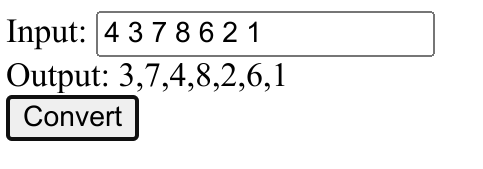
\includegraphics[width=10cm]{1/out.png}
\end{figure}

\newpage
\section*{Question 2}
The problem to rearrange positive and negative numbers in an array .
Method: This approach moves all negative numbers to the beginning and positive
numbers to the end but changes the order of appearance of the elements of the array.
Steps:
\begin{enumerate}
    \item Declare an array and input the array elements.
    \item Start traversing the array and if the current element is negative, swap the
          current element with the first positive element and continue traversing until all
          the elements have been encountered.
    \item Print the rearranged array.
\end{enumerate}
\textbf{Test case:}
\begin{lstlisting}
    Input: 1 -1 2 -2 3 -3
    Output: -1 -2 -3 1 3 2
\end{lstlisting}
\subsection*{Code}
\lstinputlisting[language=html]{2/index.html}
\newpage
\subsection*{Output}
\begin{figure}[H]
    \centering
    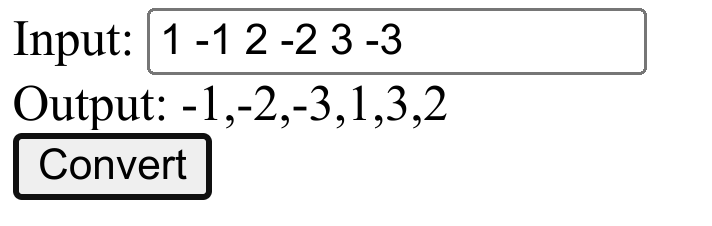
\includegraphics[width=10cm]{2/out.png}
\end{figure}

\newpage
\section*{Question 3}
Q3: Program to find all the patterns of \lstinline{0(1+)0} in the given string.
Given a string containing 0's and 1's, find the total number of \lstinline{0(1+)0}
patterns in the string and output it.
\lstinline{0(1+)0} - There should be at least one '1' between the two 0's. \\
For example, consider the following string.
\begin{lstlisting}
Input: 01101111010
Output: 3
\end{lstlisting}
\textbf{Explanation:}
\begin{lstlisting}
01101111010 - count = 1
01101111010 - count = 2
01101111010 - count = 3
\end{lstlisting}
Step to find all the patterns of \lstinline{0(1+)0} in the given string
\begin{itemize}
    \item Input the given string.
    \item Scan the string, character by character.
    \item If the given pattern is encountered, increment count.
    \item Print count.
\end{itemize}
Program to find all the patterns of \lstinline{0(1+)0}W
\subsection*{Code}
\lstinputlisting[language=html]{3/index.html}
\newpage
\subsection*{Output}
\begin{figure}[H]
    \centering
    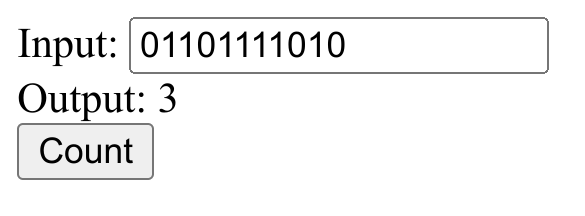
\includegraphics[width=10cm]{3/out.png}
\end{figure}

\newpage
\section*{Question 4}
Write a Java script program to o find all pairs of elements in an Array whose sum
is equal to a given number.
\begin{lstlisting}
Array numbers= [4, 6, 5, -10, 8, 5, 20], target=10
Output :
Pairs of elements whose sum is 10 are:
4 + 6 = 10
5 + 5 = 10
-10 + 20 = 10
\end{lstlisting}
\subsection*{Code}
\lstinputlisting[language=html]{4/index.html}
\newpage
\subsection*{Output}
\begin{figure}[H]
    \centering
    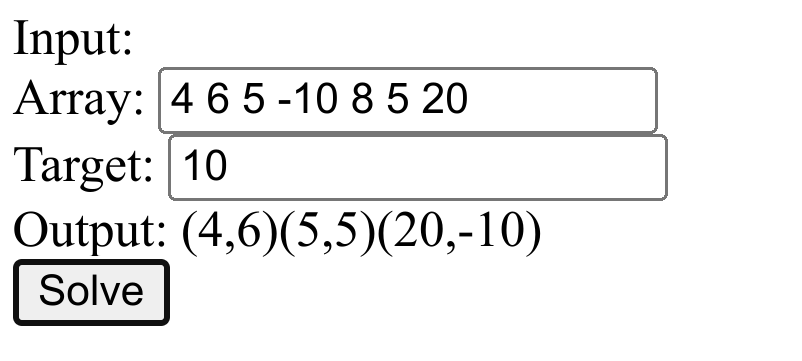
\includegraphics[width=10cm]{4/out.png}
\end{figure}

\newpage
\section*{Question 5}
Given two sorted arrays A and B of size p and q to merge elements of A with B
by maintaining the sorted order i.e. fill A with first p smallest elements and fill B with
remaining elements.
\textbf{Example:}
\begin{lstlisting}
Input :
    int[] A = { 1, 5, 6, 7, 8, 10 }
    int[] B = { 2, 4, 9 }
Output:
Sorted Arrays:
    A: [1, 2, 4, 5, 6, 7]
    B: [8, 9, 10]
\end{lstlisting}
\subsection*{Code}
\lstinputlisting[language=html]{5/index.html}
\newpage
\subsection*{Output}
\begin{figure}[H]
    \centering
    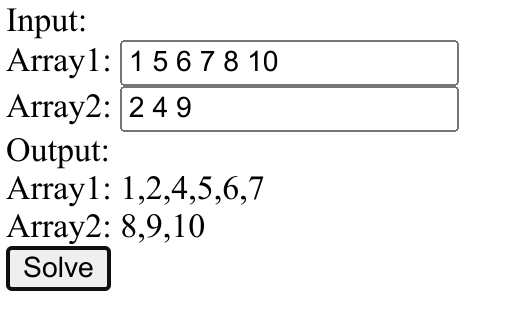
\includegraphics[width=10cm]{5/out.png}
\end{figure}
\end{document}
